%!TEX options=--shell-escape
\documentclass[tikz]{standalone}
\usepackage[T1]{fontenc}
\usepackage[utf8]{inputenc}
\usepackage{xcolor}
\usepackage{amsmath}
\usepackage{amssymb}
\usepackage{hyperref}
\usepackage{accsupp}    
\usepackage{graphicx}
\usepackage{mathtools}
\usepackage{pagecolor}
\usepackage{amsmath} % for \dfrac
\usepackage{tikz}
\tikzset{>=latex} % for LaTeX arrow head
\usepackage{braket}
\usepackage{pgfplots} 
\usepackage[edges]{forest}
\usetikzlibrary{patterns, backgrounds, arrows.meta}
\setlength{\parindent}{0cm}
\setlength{\parskip}{1em}

\usetikzlibrary{patterns}

\begin{document}
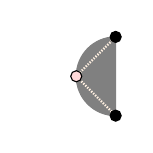
\begin{tikzpicture}[]
   
    \draw[gray, fill=gray] (0, 0) to [bend left=45] (-0.5, 0.5) to [bend left=45](0, 1) --cycle ; 



    % X Lattice
        \draw[thick, dash pattern={on 0.5pt off 0.5pt on 0.5pt off 0.5pt}, yellow!40!red!10] (0, 0) -- (-0.5, 0.5) -- (0, 1);

    \filldraw[opacity=0] (0, 0) circle[radius=2pt] node[font=\tiny] {};

    \foreach \y in {0, 1}{
            \filldraw[draw=black] (0, \y) circle[radius=2pt] node[font=\tiny] {};
        }
    \filldraw[draw=black, opacity=0] (-1, 0) circle[radius=2pt] node[font=\tiny] {};
    \filldraw[draw=black, fill=pink!60] (-0.5, 0.5) circle[radius=2pt] node[font=\tiny] {};


\end{tikzpicture} 
\end{document}

